\documentclass[tikz,border=3pt]{standalone}
\usepackage[utf8]{inputenc}
\usepackage[T1]{fontenc}
\usepackage{lmodern}
\renewcommand{\familydefault}{\sfdefault}
\usepackage{sansmath}\sansmath
\usepackage{chemfig}
\usepackage{pgfplots}\pgfplotsset{compat=1.18,/pgf/number format/use comma,/pgf/number format/1000 sep={.}}
\usetikzlibrary{arrows.meta,calc,positioning,decorations.pathmorphing,patterns}
% paleta del sitio
\definecolor{nar}{HTML}{E8680C}\definecolor{narc}{HTML}{FFB35C}\definecolor{hielo}{HTML}{FFF3E8}
\definecolor{tinta}{HTML}{1D1D1F}\definecolor{gris}{HTML}{6E6E73}\definecolor{lila}{HTML}{7C5CF0}
\definecolor{azul}{HTML}{2F6FD6}\definecolor{menta}{HTML}{17A673}\definecolor{coral}{HTML}{E8342A}
\begin{document}
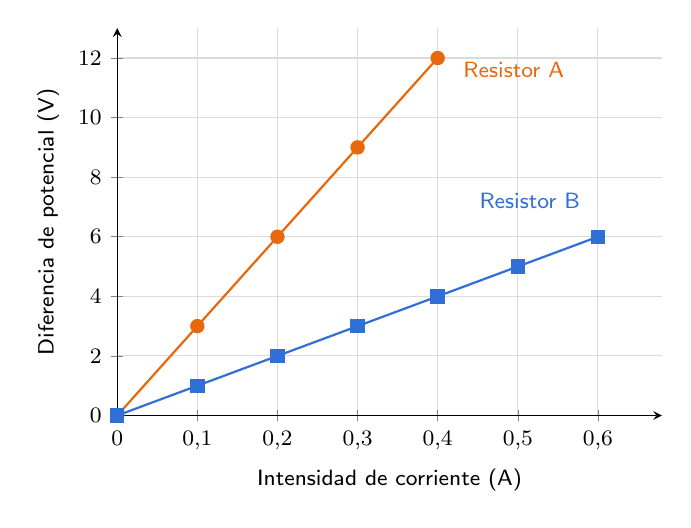
\begin{tikzpicture}[font=\footnotesize]
\begin{axis}[width=8.5cm,height=6.5cm,xmin=0,xmax=0.68,ymin=0,ymax=13,xtick={0,0.1,0.2,0.3,0.4,0.5,0.6},ytick={0,2,...,12},grid=major,grid style={gris!25},
  xticklabel style={/pgf/number format/fixed,/pgf/number format/precision=1},
  xlabel={Intensidad de corriente (A)},ylabel={Diferencia de potencial (V)},axis lines=left,every axis plot/.append style={thick}]
\addplot[nar,mark=*,mark size=2.2pt] coordinates {(0,0)(0.1,3)(0.2,6)(0.3,9)(0.4,12)};
\addplot[azul,mark=square*,mark size=2.2pt] coordinates {(0,0)(0.1,1)(0.2,2)(0.3,3)(0.4,4)(0.5,5)(0.6,6)};
\node[text=nar,anchor=west] at (axis cs:0.42,11.6) {Resistor A};
\node[text=azul,anchor=west] at (axis cs:0.44,7.2) {Resistor B};
\end{axis}
\end{tikzpicture}
\end{document}
